\chapter{UCNA Analysis}
\label{ch:UCNA_Analysis}
%%%%%%%%%%%%%%%%%%%%%%%%%%%%%%%%%%%%%%%%%%%%%%%%%%%%%%%%%%%%%%%%%%%%%%%%%%%%%%%
%%%%%%%%%%%%%%%%%%%%%%%%%%%%%%%%%%%%%%%%%%%%%%%%%%%%%%%%%%%%%%%%%%%%%%%%%%%%%%%
%%%%%%%%%%%%%%%%%%%%%%%%%%%%%%%%%%%%%%%%%%%%%%%%%%%%%%%%%%%%%%%%%%%%%%%%%%%%%%%

\iffalse
Designing an experiment and collecting the right data are non-trivial alone,
but interpreting the results lends itself to a whole new train of thought.
The rest of this thesis is spent describing the details of such an
analysis, with this chapter summarizing important aspects,
such as terminology to be used later and the
model used to characterize our detector response.
\fi

This chapter is dedicated to introducing important aspects of the analysis that
is not strictly tied to calibrations and asymmetry extraction, but rather
data collection and processing to turn raw detector signals into values that
can be calibrated and analyzed. 





%--------------------------------------------------------------

\section{Outline of Analysis Steps}

To preface the rest of this chapter, we can highlight
the general process of the analysis beginning with a raw detector
ADC value from each PMT and finishing with an asymmetry.
Below are the general steps:

\begin{itemize}
\item Determine pedestals for each PMT and subtract the pedestal from each data event.
\item Measure the gain of each PMT and divide the drifts out of the signal.
\item Apply a PMT-by-PMT calibration to determine the expected position dependent
  energy deposited in the scintillator
  for each event.
\item Correct for the position dependent response of each PMT
  to return a visible energy as seen by each PMT, $E_{\mathrm{vis},i}$.
\item Combine the four PMT energies into a single deposited energy, $E_{\mathrm{vis}}$.
\item Convert this combined estimate of the energy deposition to a final
  reconstructed energy, $E_{\mathrm{recon}}$, to use in analysis.
\item Calculate an asymmetry and apply all systematic corrections.
\end{itemize}

It is important to point out early on the difference between $E_{\mathrm{vis}}$ and
$E_{\mathrm{recon}}$. The deposited or visible energy, $E_{\mathrm{vis}}$, is the energy
physically deposited in the
scintillator by a particle, while the reconstructed energy, $E_{\mathrm{recon}}$, is an estimate of
the true initial energy of an event. The two are different due to the electron losing energy
as it traverses through the windows of the decay trap, the windows of the MWPC,
the MWPC itself, and the dead layer of the scintillator. Of course the analysis could be
done in terms of $E_{\mathrm{vis}}$, but it is more convenient to express the results
in terms of the true electron energy spectrum, and also the energy dependent theory modifications
are in terms of the true initial energy of an event.


\section{Energy Response from Detector Response} \label{sec:EnergyResponse}
Following the process outlined in the previous section, we can derive an
expression which takes a detector signal to an energy estimate for each PMT.
The visible energy $E_{\mathrm{vis},i}$ deposited
in the scintillator as seen by a single PMT $i$ for an event at position $(x,y)$ 
is given by the following: 

\begin{equation} \label{eq:EvisResponse}
E_{\mathrm{vis},i} = \eta_i^{-1}(x,y) \cdot f_i\Big[ \Big( \mathrm{ADC}_i - p_i(t) \Big) \cdot g_i(t) \Big]  ,
\end{equation}

\noindent where 
\begin{align*}
&f_i = \textrm{linearity relation from ADC channels to Energy,}\\
&\eta_i(x,y) = \textrm{PMT correction factor for position dependence,} \\
&p(t) = \textrm{mean pedestal value for PMT } i,\\
&g(t) = \textrm{gain correction factor for PMT }i.
\end{align*}

This expression is exact in the case where all values are determined with infinite
precision and without stochastic fluctuations. Unfortunately, each parameter on the right
side of this equation is either stochastic in itself (as is the ADC response), or it was
determined via observation of a stochastic process (the gain and pedestal), and so
the underlying value for any given event may not be the same as the value applied in the
above expression. Thus what we
really resolve is an approximation to the energy, which comes with some uncertainty. This
uncertainty will be addressed later in section \ref{ssec:energyRecon}.
For the time being, keep in mind the above list of
input parameters which take us from an ADC signal (detector signal) to an energy signal. 

\subsection{Combining PMT Responses}

\subsection{$E_{\mathrm{vis}}$ to $E_{\mathrm{recon}}$}



\section{Time-dependent Detector Corrections}

Obviously the system is not immune to drifts in signals due to variations
in time. There are many sources of such drifts, ranging from simple
electronic noise to changes in temperature. We deal with such time-dependent
effects using pedestal subtraction, gain correction, and constant monitoring
of backgrounds.

\subsection{Pedestal Subtraction}
The pedestal is a measure of the inherent detector signal, or baseline, 
upon which all other data signals lie. In terms of PMT signals, you can imagine 
the pedestal as a non-zero ADC value corresponding to zero input, or an offset.
You might say that the experiment can be run without caring about an offset
because the calibration will take this into account, which would be the case 
if the pedestals were constant or if we calibrated each run against itself, but 
neither is the case. We use a collection of subsequent runs to form our 
calibration sets, and these sets then calibrate data which is often taken hours,
or even days, earlier or later. Thus changing pedestals can be worrisome, and care
must be taken to determine the pedestals and subtract them from data.

To determine a pedestal, events must be chosen where there was a global trigger, but
the PMT of interest does not trigger and preferably there is no signal
whatsoever in the scintillator on that side. Obvious choices for these events are
UCN monitor triggers, opposite side two-fold PMT triggers, and high-threshold $^{207}\mathrm{Bi}$
pulser triggers from other PMTs. Once there is a global trigger, we can use the individual TDC
to ensure there was no individual trigger, and the events can be 
histogrammed for the PMT of interest. This leads to pedestals like those seen in
figure \ref{fig:peds_ind}. The mean of this peak can be taken as the average pedestal for a single run,
and this value can be 
subtracted from every subsequent reading of this PMT.

One interesting thing to note is that the discriminators, which determine whether
a component triggers,
for all PMTs are housed 
together, which leads to correlations between the PMT triggers. In a perfect world, 
each PMT would have one pedestal, and that pedestal wouldn't care about other PMT's signals.
Instead, what we see in figure \ref{fig:peds_types} is that the pedestals
can be dependent on the type of events that are chosen 
to construct the pedestal. This indicates that the pedestal for one PMT may be dependent
on the signal present in another PMT. These shifts are important as a
pedestal shift of ~5-10 channels maps to an offset of roughly
~5-10 keV, as the PMTs show roughly 1:1 correspondence between ADC and keV.

The influence of event type on pedestal values means we must carefully choose which events
to use when calculating the pedestal.
The best choice would be UCN monitor events due to there being zero signal 
in the electronics box housing the PMT electronics, and these thus would give
the cleanest measurement of the PMT pedestal.
These are unfortunately the first event type we can eliminate as they are only present
during $\beta$-decay runs (when UCN are produced and thus create UCN monitor triggers)
and not during calibration runs (taken during the day when the beam is off). 
Of the remaining two options, the choice was made to use the
two-fold PMT triggers from the opposite detector rather than $^{207}\mathrm{Bi}$ pulser
events. The choice is somewhat arbitrary, because what is important is that we choose
a consistent subset of data for both calibration and $\beta$-decay data, but the
opposite side two-fold triggers do better represent the baseline present in each PMT
for data events when compared to the much higher signal present from the $^{207}\mathrm{Bi}$
pulser.


\begin{figure}[h] 
\centering

\includegraphics[scale=.25]{3-UCNAAnalysis/ImageHolder.pdf}
\caption{Pedestal values for a $\beta$-decay run determined using different 
types of events to illustrate the cross-talk between PMTs. (UCN Monitors, 
Bi triggers, Opposite side triggers, same side 2-fold triggers. Also shown 
is the dependence of the pedestal on which PMT triggers in the Bi Pulser. NOTE:
Choose West PMT4 in an early 2012/2013 beta run) }
\label{fig:peds_types}
\end{figure}

\begin{figure}[h] 
\centering

\includegraphics[scale=.25]{3-UCNAAnalysis/ImageHolder.pdf}
\caption{Example pedestals from all 8 PMTs}
\label{fig:peds_ind}
\end{figure}

With the event type chosen, we extract the mean and RMS of the pedestal peak (see figure
\ref{fig:peds_ind}) for each PMT in every run. The pedestal mean (referred to as simply
the pedestal) is then subtracted from the ADC values for all events. This effectively
removes the time-dependent baseline from the detector signals. The time dependence of
the pedestals can be seen for the East PMTs from 2011-2012 in figure \ref{fig:peds_timeDep}.
Most of the PMTs have pedestals which remain quite stable, but PMT East 3 shows the
importance of a run-by-run pedestal subtraction.

\begin{figure}[p]
\centering
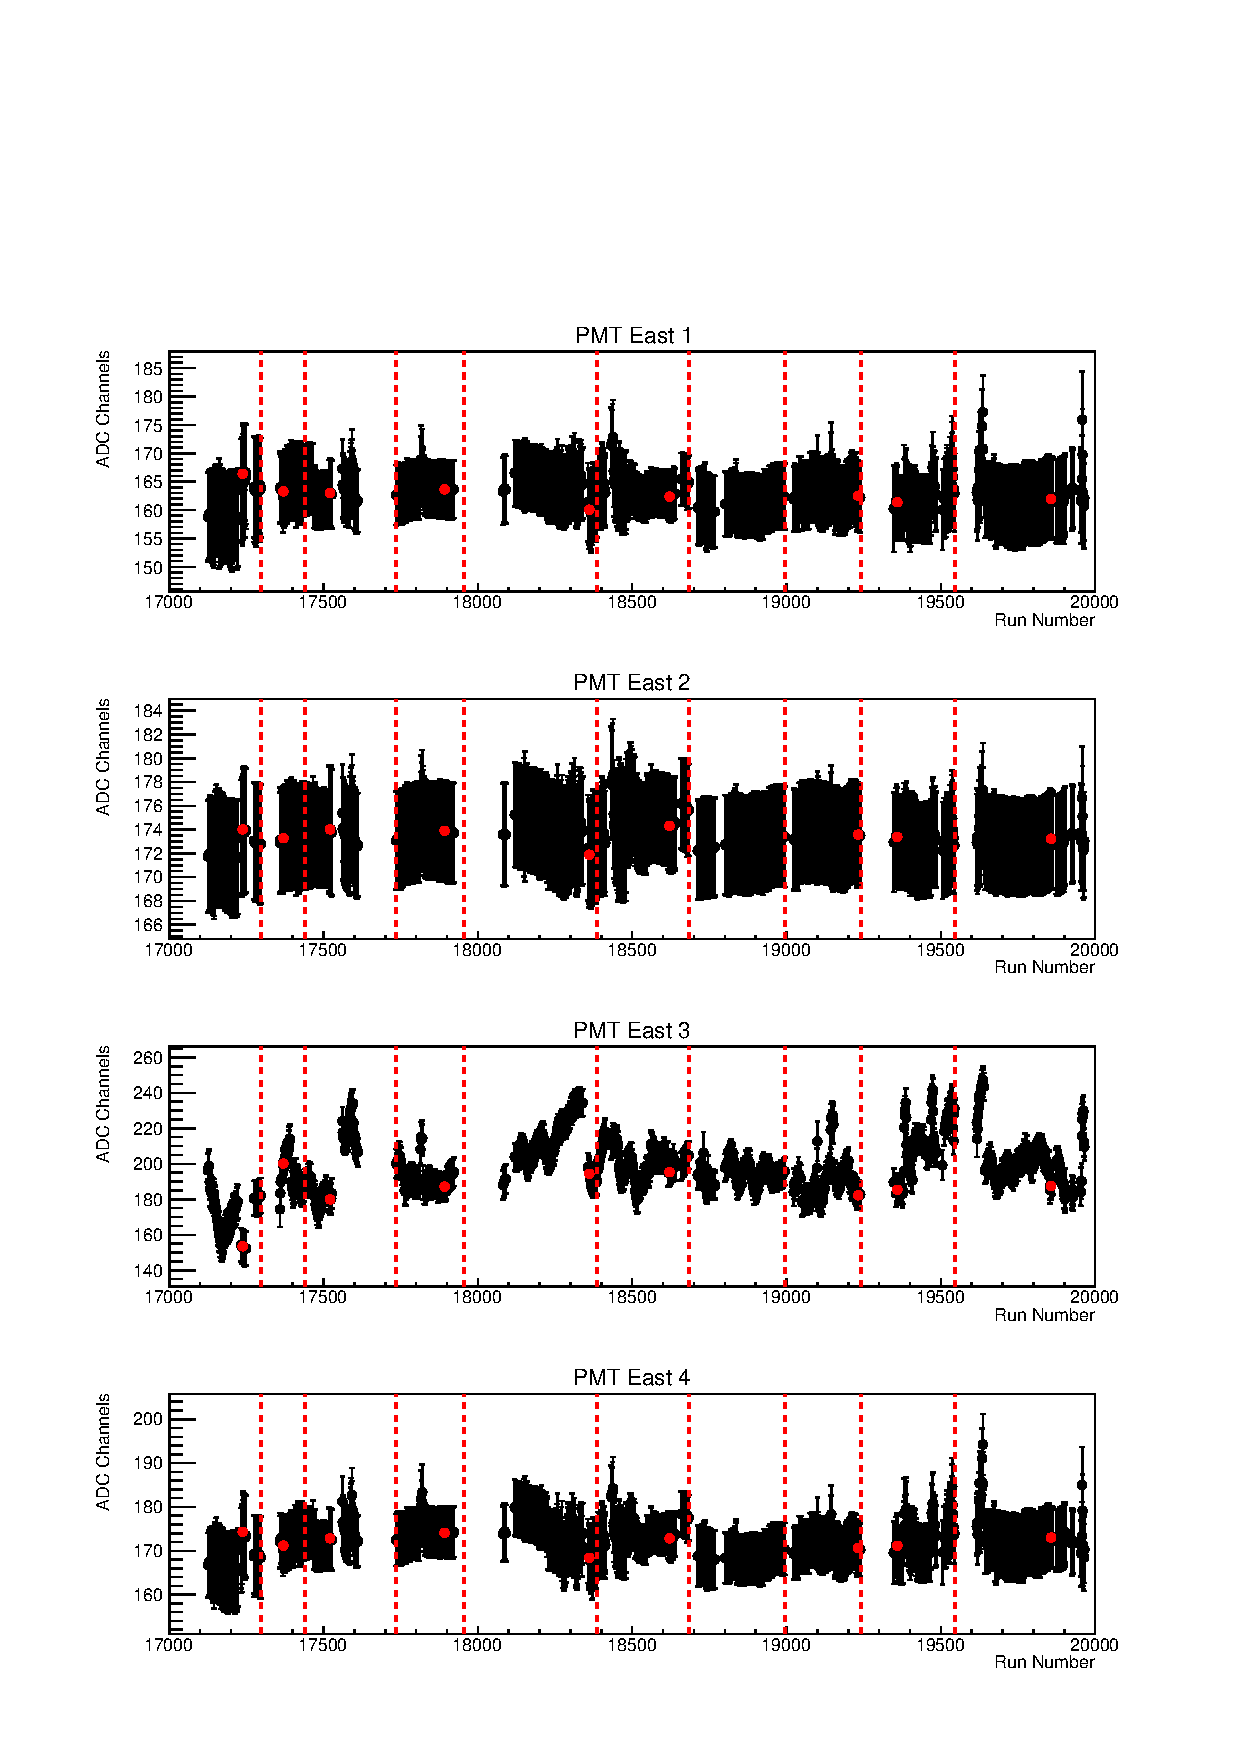
\includegraphics[page=1,scale=0.8]{3-UCNAAnalysis/2011-2012_pedestals.pdf}
\caption{Pedestal means as a function of run number for 2011-2012 East Detectors. Error bars are the
  RMS of the measured pedestal. The red lines indicate what ranges of runs belong to
  different calibration periods, and the red marker is the calibration reference run,
  which will be discussed in later sections.}
 \label{fig:peds_timeDep}
\end{figure}

\begin{figure}[p] 
\centering
\includegraphics[page=2,scale=0.8]{3-UCNAAnalysis/2011-2012_pedestals.pdf}
\caption{Pedestal means as a function of run number for 2011-2012 West Detectors. Error bars are the
  RMS of the measured pedestal. The red lines indicate what ranges of runs belong to
  different calibration periods, and the red marker is the calibration reference run,
  which will be discussed in later sections.}
\label{fig:peds_timeDep}
\end{figure}

\subsection{Gain Correction}

\subsubsection{$^{207}\mathrm{Bi}$ Pulser}
%The goal of the $^{207}\mathrm{Bi}$ gain monitoring pulser system is to create a standard
%candle type signal present in all PMTs to be tracked over time. 
The primary gain monitoring system consists of a small amount $^{207}\mathrm{Bi}$
deposited within a small block of scintillator. The scintillator was surrounded by
light reflecting material on three sides, with the fourth side covered with an optical
attenuator to attempt to match the light output of the \~1~MeV conversion line in the $^{207}\mathrm{Bi}$
to the light output of 1~MeV of energy deposited in the detector scintillator. The pulser was then
attached directly to the PMT next to where the light guides attached to the PMT.
To allow for a single-PMT high threshold trigger, the signal was split off to a different
discriminator than the one used when determining a two-fold trigger. These high threshold
discriminators then allowed for pulser triggers with a distinct pulser identification \cite{mpmThesis}.

An unfortunate but low impact issue with the pulser involves the amount of attenuation applied to the
pulser signal. The pulser peak lies well beyond the equivalent of 1~MeV of light as would be produced
in the detector scintillator, and therefore far outside the range of the $\beta$-decay spectrum. This
is not a serious issue as the PMTs seem to be quite linear, so even a peak well outside the
energy range of interest should suffice.

\begin{figure}[h] 
\centering

\includegraphics[scale=.25]{3-UCNAAnalysis/ImageHolder.pdf}
\caption{Example pedestals from all 8 PMTs}
\label{fig:biPulser}
\end{figure}

The $^{207}\mathrm{Bi}$ pulser peak is fit on a run-by-run basis, allowing for gain corrections on the time
scale of a single run. The fit was done iteratively, with the initial guesses for mean and fit range determined
by stepping backwards from the last bin and using a self-written algorithm to search for the peak. Then the the peak
was fit five times consecutively, with each successive fit being fed the previous fit's mean and sigma. This
made sure the fit converged as best as possible on the mean of the pulser peak. An example pulser peak and fit
can be seen in figure \ref{fig:biPulser}.

The method for applying the gain correction is as follows. First, a reference gain must be determined
to normalize all other gains against. This was chosen to be what is called the ``reference run'', and it
typically consists of a manually inspected source run within each source calibration period. The gain factor
is then calculated as the ratio of the pulser peak in a given run divided by the pulser peak in the reference
run, or
%
\begin{equation}
  g_i = \frac{\mu_i}{\mu_{\mathrm{ref}}}
\end{equation}
%
This automatically defines the gain of the reference run to be $g_{\mathrm{ref}}=1$. Then all other runs which are
calibrated by a certain run period have gain factors which vary based on the fitted pulser value. The time
dependence of the gain values in 2011-2012 can be seen in figures \ref{fig:2011-2012pulser_East}
and \ref{fig:2011-2012pulser_West}. The behavior is similar in 2012-2013.

Some problems with the $^{207}\mathrm{Bi}$ pulser did occur. There were several periods where the pulser
simply did not work for a certain PMT. This was always limited to a single PMT not working, and when this
was the case the PMT without a pulser signal was not used when reconstructing the energy. This has
minimal effect on the energy reconstruction though, as the ``bad'' PMT is still used when determining
a two-fold trigger, and the remaining three PMTs contain sufficient information for reconstructing the
energy deposited. Periods where $^{207}\mathrm{Bi}$ pulser information is missing are evident in
figures \ref{fig:2011-2012pulser_West} where there is missing data for certain PMTs over extended ranges.
It should be noted that in 2012-2013, West PMT4 never had a functioning pulser.

\begin{figure}[p] 
  \centering
  \includegraphics[page=3,scale=.8]{3-UCNAAnalysis/2011-2012_gain.pdf}
  \caption{Gain factors, $g_i$, as a function of run number for 2011-2012 East Detectors.
    The red lines indicate what ranges of runs belong to
    different calibration periods, and the red marker is the calibration reference run.}
  \label{fig:2011-2012pulser_East}
\end{figure}

\begin{figure}[p] 
  \centering
  \includegraphics[page=4,scale=.8]{3-UCNAAnalysis/2011-2012_gain.pdf}
  \caption{Gain factors, $g_i$, as a function of run number for 2011-2012 West Detectors.
    The red lines indicate what ranges of runs belong to
    different calibration periods, and the red marker is the calibration reference run.}
  \label{fig:2011-2012pulser_West}
\end{figure}

\subsubsection{Endpoint Stabilization}

There are unexplained longer term gain fluctuations that do not seem to be captured by the
$^{207}\mathrm{Bi}$ gain monitoring system that can be seen by monitoring the endpoint of the
$\beta$-decay spectrum. These are corrected by fitting the endpoint using a Kurie plot for each
PMT and comparing to the expected endpoint from simulation. Then a secondary gain correction
factor can be applied to match the endpoint of each PMT to the expected endpoint. The endpoints
before and after such a correction can be seen in figure \ref{fig:endpoints}, where the
large deviation over runs xxx-xxx was corrected.



\subsection{Time-dependent backgrounds}
Background events which may have some time dependence are removed from the analysis
via dedicated background runs that accompany every $\beta$-decay run.
Subtracting these background rates from the data rates accounts for backgrounds
with roughly a one hour time variation.
Any backgrounds that vary at the sub one hour level may go unnoticed, but
with a signal to background better than 50:1 the contribution from such is minimal.
The background run scheme will be addressed later in this chapter, with the background
subtraction addressed in chapter 5. 

\section{Trigger Thresholds}

Looking ahead to the detector response model that will be implemented in the
simulation to take well-defined simulated particle energies and transform them into
signals that mimic those from our detectors, we here define the determination
of the trigger thresholds for each PMT. The PMT does not trigger at a single
predefined ADC value (like a step function), but instead a smooth transition
from zero trigger probability to trigger probability of one occurs. This is primarily
due to the random nature

An integral piece of the PMT Response Model from section \ref{sssec:pmtModel} 
is the sampling of the threshold functions to determine whether or not a detector
triggered. I'll repeat here that a 2-fold PMT trigger from one of the two electron
detectors is required to create a global electron trigger from the DAQ. In simulation
we only see the energy deposition as a whole from an individual scintillator, and then
we model the four-pmt response for that side. At low energies, this response is 
intimately entwined with the trigger threshold.

\subsection{General Model for Trigger Determination} \label{ssec:genTrigModel}
Obviously one must rely on data to determine the trigger thresholds of a detector, since
the non-step-functional shape is directly related to the stochastic nature 
of the detector and electronics. If we knew with infinite precision and 
accuracy the signal produced in a detector
and could read out the response in real time with infinite precision, 
there wouldn't be muchneed for a model to estimate trigger probabilities. 
Instead, to understand the trigger threshold, a functional 
form for the probability of a trigger need be determined using real data which may or 
may not have created a trigger in a detector/PMT. 

The most important part of determining the trigger threshold shape for 
any detector is the availability of data which was collected no matter if 
the detector or component (PMT) produced a trigger. If such a subset of 
data is available and plentiful, it is straightforward to estimate
the trigger probability by binning the data in some unit proportional to 
energy (whether in energy or something like it isn't important) and taking 
the bin-by-bin ratio of those events that triggered to all of the events in the 
sample. Plotting these ratios as a function of whatever metric was chosen tells 
you how probable an event of some value is to create a trigger.
Once you have mapped this probability, you can then sample these curves within 
simulation to apply your true trigger threshold to simulated data.

The not-so transparent part of the trigger probability comes when calculating the error of the estimate in each bin, since the numerator and denominator in the ratio are correlated. But as demonstrated in \cite{casadei2009efficiency}, the ROOT analysis framework handles efficiency errors effectively via use of Bayesian Statistics. 

PUT IN DISCUSSION OF BAYESIAN STATISTICS FOR EACH BIN AND ASYMMETRIC ERROR BARS
AND CONFIDENCE LIMITS.

\subsection{Trigger Data Selection}
As mentioned before, the data used for constructing trigger thresholds must not be 
biased towards triggering the PMT of interest. Thus that PMT must not be a mandatory 
component of the global trigger for that event, so care must be taken to choose only 
events which would trigger regardless of the behavior of the PMT of interest. One
other stipulation placed on these events is that they have an opportunity to 
deposit energy in a particular scintillator. The best choice of events which 
satisfy these conditions are those which have a two-fold trigger on the opposite side 
and then backscatter and those which trigger at least three PMTs on the side of 
interest, which guarantees that the scintillator would have triggered with or without 
whatever PMT one is interested in.	

\subsection{Determining the Trigger Probability}
One option for determining the trigger probability function (and probably the 
most straightforward) is to calculate the trigger probability for an entire detector as 
a whole as a function of the energy deposited by an event. What you get is a 
function that provides the probability that an event of energy $ E_i $ 
produces some sort of trigger, either 2-fold, 3-fold, or 4-fold, in that 
detector. Initially this method was used for sake of simplicity, and it produced 
reasonable agreement between simulation and data, but there is one 
glaring concern: Determining this trigger function from data requires that the data be 
calibrated first. At first glance this may not seem like much of an issue, but the 
calibration hinges upon the 
simulated peaks at low energy, which in turn rely on the trigger functions. This 
cyclical dependence hinders one from truly understanding any discrepancy between 
simulation and data at low energies, which is exactly the reason this method was 
abandoned.  

Instead, similarly to previous analyses, we decided to calculate the trigger
function on a PMT-by-PMT basis as a function of ADC channels above threshold. This
encompasses a true characteristic of each component of the detector rather than some
average effect as seen by a detector package, which is what the aforementioned 
method produces. A typical trigger threshold is seen in figure \ref{fig:trigger_thresh}.
As illustrated in section \ref{ssec:genTrigModel}, the ratio of triggering events
to all events was taken in each ADC bin and then fit using the method described
in the following section.
  

\begin{figure}[h] \label{fig:trigger_thresh}
\centering

\includegraphics[scale=.25]{3-UCNAAnalysis/ImageHolder.pdf}
\caption{Typical trigger threshold functions with Bayesain errors 
applied. }
\end{figure}

\subsubsection{Functional Fit of the Trigger Threshold}


%-----------------------------------------------------------


\section{Wirechamber Position Reconstruction}

%----------------------------------------------------


\section{Position Dependent Light Transport Maps}

As mentioned in the experimental description, each PMT is coupled to a quadrant of
the scintillator and collects the most light from this quadrant. The light collection
is therefore position dependent, and an individual PMT will receive a different
amount of light for an event of energy $E_i$ depending on where that event strikes
the scintillator. To properly map the PMT signal to energy, this position dependence
must be accounted for on a PMT-by-PMT basis. The collection of values which correct for this
dependence will appropriately be called position maps from here on.


\subsection{Activated Xenon}

To map the position response of the scintillator, signals must be present across the
entire face of the detector. The $\beta$-decay spectrum
is an obvious option, and was used for these position maps prior to 2010,
but the event rate is low when divided into small position bins across the scintillator.
Prior to running in 2010, a method using activated xenon was developed to provide
a higher event rate and also full fiducial coverage.

The xenon is activated by placing a small amount of natural xenon in the volume that
normally holds the $\mathrm{SD}_2$ source, freezing it, and then exposing it to the moderated
neutron flux for several minutes. This produces a plethora of radioactive isotopes
with various half-lives. The xenon is then warmed up to a gas and stored. The gas
is then released into spectrometer during position mapping periods, and the decay products
are detected \cite{mpmThesis}. The various radioactive isotopes provide several features to fit across the entire
detector surface.

The spectral shape of the activated xenon changes with time due to the different half-lives
of the isotopes, but this is not a concern as the PMT will see the same shape at all positions
across the detector, just with different ADC scales due to the position dependence of the light
collection. Therefore one only needs to choose a feature of the spectrum to fit in different
positions to map the relative response.

\subsection{Position Maps}

The scintillator is divided into a grid of $5\times5\mathrm{~mm}^2$ squares (in the 1~T
decay trap coordinates) with one square directly in the center,
and the xenon events are collected for each of these ``pixels''. A key feature
from the spectrum is then chosen and fit in every pixel, with the position dependent response
factor in pixel $i$ for a single PMT defined as
%
\begin{equation}
  \eta_i = \frac{Q_i}{Q_0},
\end{equation}
%
where $Q_i$ is the fitted ADC value of the feature in pixel $i$ and $Q_0$ is the fitted ADC value of the
feature in the center pixel. This normalizes the position response for a PMT to the center pixel. The
position response at some position $(x,y)$ is then calculated via a two-dimensional Catmull-Rom
cubic interpolating spline \cite{catmull1974}. The same interpolation is used in the plots of the
position dependence in figure \ref{fig:posmaps}.

\begin{figure}[h] 
\centering
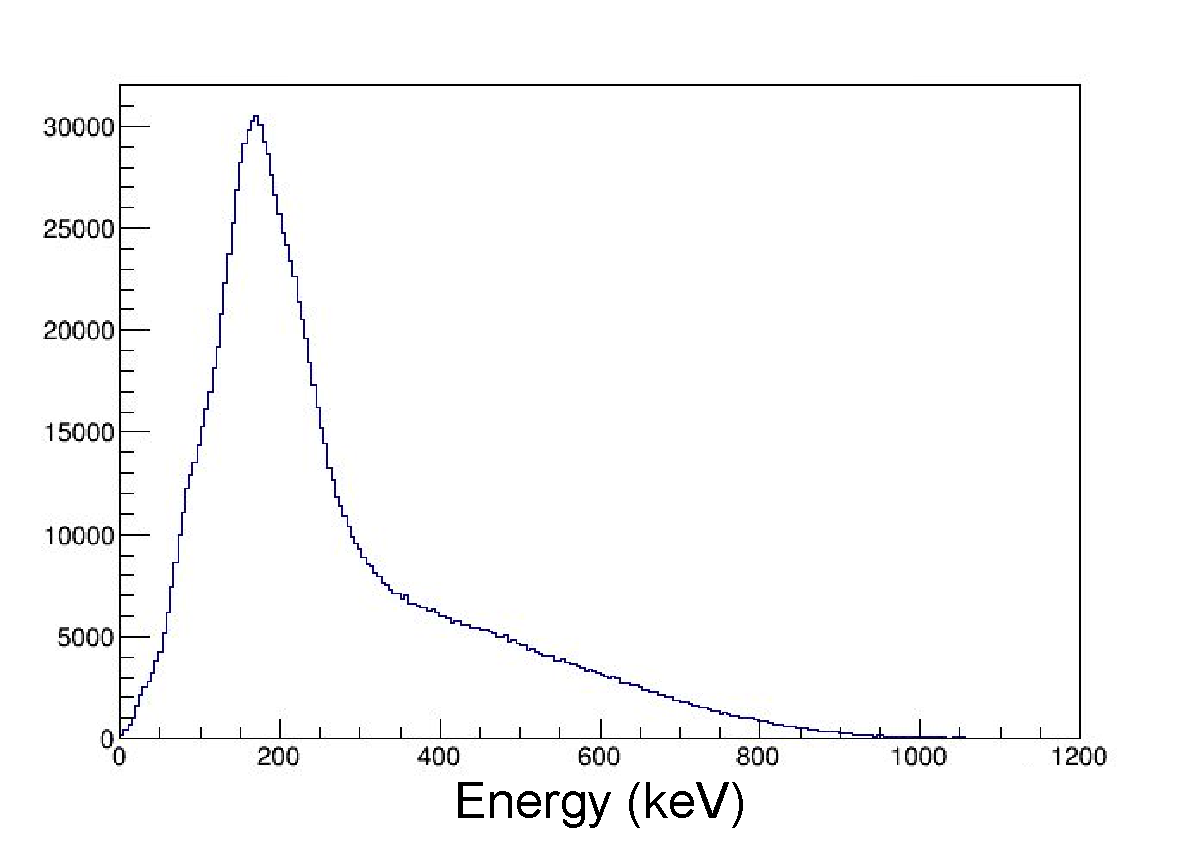
\includegraphics[scale=.5]{3-UCNAAnalysis/xenonSpectrum.pdf}
\caption{Example energy spectrum of the neutron-activated xenon used for position map determination. }
\label{fig:xenonSpectrum}
\end{figure}

A typical xenon energy spectrum can be seen in figure \ref{fig:xenonSpectrum}. The two obvious features one could
fit are the peak between 100~keV and 200~keV or the 915~keV $\beta$-decay endpoint. The peak is a
superposition of several isotopes, while the endpoint comes from the
$^{135}\mathrm{Xe~}\frac{3}{2}+$ isotope. The position maps are fit in terms of pedestal and gain corrected ADC,
so unfortunately the luxury of knowing an initial guess for the feature position is not afforded as it would
be if the fit was done in the energy domain. This makes
fitting the peak more reliable upon first inspection, as the endpoint fit (done via a Kurie fit as described
in appendix \ref{app:kurieFit}) is more sensitive to the range of the fit especially when the spectrum is not
purely a $\beta$-spectrum. There is a problem with using the peak though, as areas with low light collection
for a given PMT lose a portion of the peak below the trigger threshold. This changes the feature shape
compared to regions of higher light output, thus biasing the position map. The better choice is then the
$^{135}\mathrm{Xe~}\frac{3}{2}+$ endpoint. 

The problem with fitting the endpoint in pixels with different light collection efficiencies is illustrated by
imagining that every pixel sees the same xenon energy spectrum (as in figure \ref{xenonSpectrum}), but that
the spectrum is compressed or stretched when compared to the spectrum in the center pixel depending on where
the pixel is located. Since each pixel has the same ADC range, choosing the proper fit range becomes difficult
as it is different in every pixel. To avoid this issue, a secondary feature was derived to be used as a
seed to the endpoint fit range. This secondary feature is calculated by first fitting the peak with a Gaussian
and extracting the mean ($\mu$) and sigma ($\sigma$), and then calculating the average ADC value, $\xi$, of the spectrum
from $\mu+1.5\sigma$ and beyond. Then the endpoint fit is done over the range $(\xi,2\xi)$. The range used to
calculate $\xi$ and the range over which the endpoint were fit were determined via trial and error, and produce
consistent results across the entire detector.

It should also be noted that the position maps were calculated using both the peak and the endpoint as the key
feature, and the differences are small. This is illustrated in figure \ref{fig:posmapCompare}, where the
ratio of the two methods is plotted.



%----------------------------------------------------------




\section{Calibration Overview}

\subsection{PMT Calibration}

\subsection{Wirechamber Calibration}

 


\section{Polarimetry} \label{sec:polarimetry}







